\documentclass[tikz, border=10pt]{standalone}
\usetikzlibrary{arrows.meta, positioning}

\begin{document}
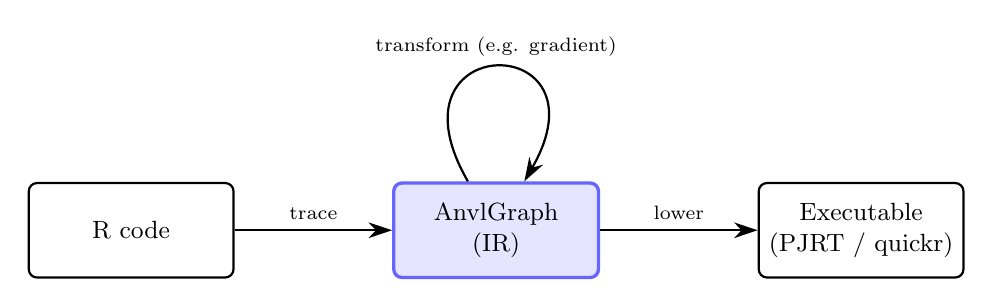
\begin{tikzpicture}[
  node distance=2cm,
  box/.style={
    draw, rounded corners=3pt, thick,
    minimum width=2.6cm, minimum height=1.2cm,
    align=center, font=\small
  },
  ir/.style={
    box, fill=blue!10, draw=blue!60, very thick
  },
  arr/.style={
    -{Stealth[length=3mm, width=2mm]}, thick
  }
]
  \node[box] (R) {R code};
  \node[ir, right=of R] (G) {AnvlGraph\\(IR)};
  \node[box, right=of G] (E) {Executable\\(PJRT / quickr)};

  \draw[arr] (R) -- node[above, font=\scriptsize] {trace} (G);
  \draw[arr] (G) -- node[above, font=\scriptsize] {lower} (E);
  \draw[arr] (G) edge [loop above, looseness=8, out=120, in=60]
       node[above, font=\scriptsize] {transform (e.g. gradient)} (G);
\end{tikzpicture}
\end{document}
